%!TEX root = ../username.tex
\chapter{Background} \label{bg}

This section contains the background information necessary to understand the project. % TODO make this more formal

%\section{Mathematical Notation} \label{bg:mathNotation}
% contains notation that may be unfamiliar to readers
% this secion may not be necessary



\section{Musical Terminology and Notation} \label{bg:musicTerminology}

In order to fully understand this project, it is important to understand the following musical terminology:

\textbf{chord}: A chord consists of several notes played as a single unit.
Most commonly, three or more notes are played simultaneously, though two notes may also constitute a chord.
Common chords are based on the major and minor scales, with variations depending on the order of the notes from lowest to highest.

\textbf{chord tone}: A note used in a chord.

\textbf{harmony}: Harmony consists of all the notes played at the same time as the melody that are not part of the melody.
In Western music, these harmonies generally follow a progression of chords based on the key that enhance the melody.

\textbf{key}: The key of a piece of music determines the chords that appear, as well as the scale the music generally follows.
Key is notated by the key signature on the music staff.

\textbf{melody}: The melody is the most prominent part, often played in the highest voice.

\textbf{non-chord tone}: A non-chord tone is a note that appears while a chord is played, but is not part of the chord.
Non-chord tones may be used to insert dissonance and drive a piece of music toward resolution.

\textbf{note}: 

\textbf{note length/rhythm}: Durations of notes used to indicate how much of each beat a note should occupy and are divided as follows:
The quarter note (\quarternote) is often the most basic division of the beat, at one quarter note per beat.
The eight note (\eighthnote) is half half the duration of the quarter note, while the half note (\halfnote) is double the duration of the quarter note, and the whole note (\fullnote) is four times the duration.
The names for these note lengths come from how many can fit in a common time measure.
These durations continue in ether direction, so you can have sixteenth and thirty-second notes, as well as double whole notes.
Dots can also be applied to notes to add half the duration of the base note.
For example, a dotted quarter note (\quarternote.) takes the same amount of time as three consecutive eighth notes (\eighthnote \eighthnote \eighthnote).

%\textbf{octaves}: 

\textbf{pitch classes}: When two notes have the same letter, but are not necessarily in the same octave, they have the same pitch class.
When discussing the harmonic structure of music, notes of the same pitch class are equivalent, so the octaves in which notes appear do not change the harmonic structure.

\textbf{scale}: A scale is a way of choosing which notes to include in a piece and is closely related to the concept of a key.
Scales begin on one pitch class, and ascend one octave before repeating.
Different modes have different feelings.
For example, the major mode (Ionian) sounds more bright and happy, while the minor modes (Aeolian, Dorian, and Phrygian) sound more dark and sad.

\section[Markov Chains]{Markov Chains} \label{bg:markov}

Intuitively, we may think of a Markov chain as a machine that accepts some former state or states of a system and produces the next state in the system.
The decision of what the next state should be is based on probabilities of transitioning to different states from the current state of the system.

\subsection{Definition} \label{bg:markov:definitions}

More formally, a \textit{Markov chain} is a type of discrete-time stochastic process, which means a Markov chain is a sequence of random variables $\boldsymbol{X} = \{X_{n} | n \in I\}$ for some index set $I$.
Additionally, Markov chains have the special property that they depend only on the immediate past state(s).
That is, for a first-order Markov chain at time $t$, $$P(X_{t} = j \mid X_{0} = i_{0}, \ldots, X_{t - 1} = i_{i - 1}) = P(X_{t} = j \mid X_{t - 1} = i_{t - 1})$$ for a particular possible outcome $j$ of $X_{t}$ \cite{nierhaus_algorithmic_2009}.

This idea can also extend to higher-order Markov chains.
A higher-order Markov process considers more than the single most recent state to determine the next state.
An $n$th order Markov chain uses the previous $n$ states as the input to find the next state.

\subsection{Representations} \label{bg:markov:representations}

In the case when $n = 1$, we can think of a Markov chain as a directed graph, where each state is a node, each edge is a transition between states, and the probabilities of transitioning between states are represented by the edge weights.
See Figure \ref{fig:markovGraph} for a visual representation of this idea.

\begin{figure}[h]
	\centering
	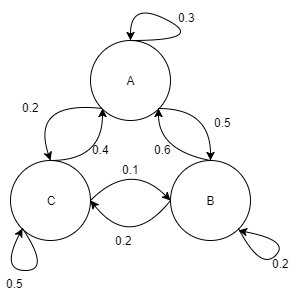
\includegraphics[width=\linewidth]{figures/markovGraph.png} % TODO: Make a better diagram
	\caption[A Markov chain represented as a graph.]{A Markov chain represented as a graph. Arrows between nodes represent transitions between nodes.}
	\label{fig:markovGraph}
\end{figure}

When implementing a Markov chain in code, however, it is perhaps easier to represent it as an $(n + 1)$-dimensional array, where $n$ is the order of the Markov chain.
We call this $(n + 1)$-dimensional array the \textit{transition matrix}.
It contains the probabilities of transitioning from one state to another.
See Figure \ref{fig:markovMatrix} for an example of the same Markov chain as in Figure \ref{fig:markovGraph} in matrix form.

\begin{figure}[h]
	\centering
	\begin{tabular}{c | c c c}
		& $A_{1}$ & $B_{1}$ & $C_{1}$\\
		\hline
		$A_{0}$ & $0.3$ & $0.5$ & $0.2$\\
		$B_{0}$ & $0.6$ & $0.2$ & $0.2$\\
		$C_{0}$ & $0.4$ & $0.1$ & $0.5$
	\end{tabular}
	\caption[A Markov chain represented as a transition matrix.]{A Markov chain represented as a transition matrix. Rows represent transitions from the labeling node to the labeling node of each column.}
	\label{fig:markovMatrix}
\end{figure}

\subsection{Limitations} \label{bg:markov:limitations}

A major limitation of Markov chains is their inability to generate truly novel output.
In order for some state to appear, a transition to that state from the previous state must appear in the source material.
% TODO define source material
That is, no truly novel transitions may appear; all transitions that appear in the output of the Markov chain must have appeared somewhere before.
Additionally, lower-order chains may produce nonsensical output, whereas a chain of sufficiently high order will exactly copy the source material.
Another limitation is that the process may get stuck in a ``local loop''.
This may happen when the chain proceeds to a state which only transitions to itself or transitions to a set of states that only transition to each other.

See Chapter \ref{markov} for more information on how Markov chains are used in this project.

%\section{Neural Networks} \label{bg:nn}
% maybe? would give brief crash course of NNs


\section{Genetic Algorithms} \label{bg:ga}
% a beief crach course on GAs
%\subsection{Definition}

In general, a \textit{genetic algorithm (GA)} is an iterative process that takes an initial population of individuals and produces a new set of individuals to become the initial population of the next generation.
This new set is produced by performing various operations on the initial population, then using a fitness function to choose the best performing individuals.
% TODO define initial population, sequences
An essential operation for GAs is mating the initial population, that is, splicing the initial individuals together to produce new sequences.
After creating the new population, we introduce mutations to keep the population from stagnating.
These mutations can include random changes or more intentional operations to improve the fitness of the individual.

To choose the new initial population, a fitness function is defined which measures how close an individual is to the desired output.
If some individuals reach a certain level fitness, they are the output of the genetic algorithm.
Otherwise, the best performing individuals become the initial population of the next generation.
This process continues until some individuals perform well enough.

See Chapter \ref{ga} for more information on how genetic algorithms are used in this project.

% TODO give a simple example here
